\chapter{Design}
\label{cha:design}

As detailed in the previous chapters, the Spoofax Language Workbench already
offers a wide variety of services to assist in developing new domain specific
languages. However, not all exposed functionality can be used easily from within
the context of a REPL, where a user wants to be able to type in some expressions
and see their results.

An example is the various transformation goals made available to the user by a
language designer. There is no such thing as a uniform ``evaluation command''
that works across all languages. Instead, each language defines its own
transform goals, of which one is an evaluation goal. Furthermore, the sequence
of processing steps needed to go from source to parsed source to a transformed
result also varies between languages. One of the main goals that the design had to
accomplish, therefore, was to expose a uniform interface for the various
transformation stages to REPL frontends.

\Cref{sec:overview} gives an overview of the product design and its components.
Afterwards, the individual components are explained in more depth.
\Cref{sec:commands} addresses the presentation of a uniform interface to
frontends by encapsulating operations in commands. \Cref{sec:function-comp}
details how commands have been decomposed into smaller functions, which allows
frontends to build their own transformation pipeline. \Cref{sec:visitor}
explains how transformation results are returned to the REPL frontends.
\Cref{sec:eval-strat} discusses the DynSem evaluation strategy. An explanation
is given as to how other evaluation strategies can be added to the existing
design to support other interpreter backends, such as Stratego.

\section{Overview}
\label{sec:overview}

As stated in \cref{ssec:goals}, one of the design goals during the project was
to keep the implementation of the REPL IDE-agnostic. To achieve this goal, the
product has been split into a backend and several frontends. The backend
interacts with the Spoofax services on behalf of the frontends. An overview of
its design can be found in \cref{fig:uml-overview}. A diagram of the complete
design can be found in \cref{cha:uml-diagram}.

\begin{figure}[h!]
  \centering
  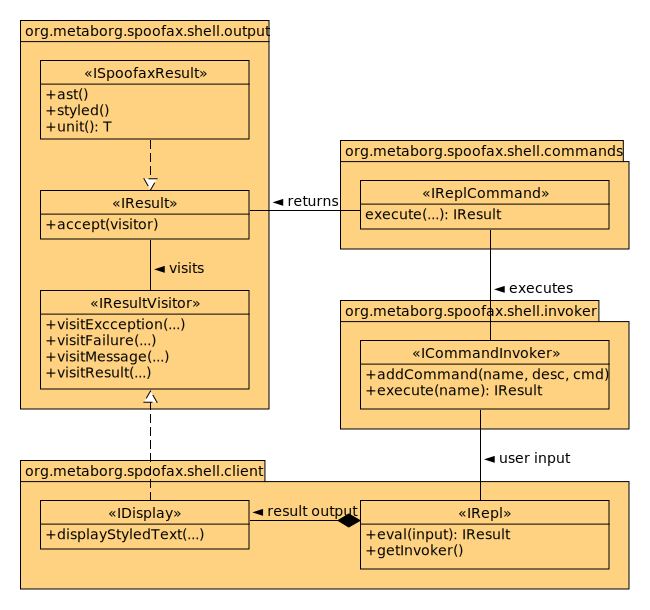
\includegraphics[width=0.75\textwidth]{uml-overview}
  \caption{An overview of the most relevant components of the backend.}
  \label{fig:uml-overview}
\end{figure}

To request and receive results from the backend, a frontend can invoke commands
by sending the command name and its parameters to the \texttt{ICommandInvoker}
in the backend. The \texttt{ICommandInvoker} will then execute the
\texttt{IReplCommand} corresponding to the command name. Every executed command
returns an \texttt{IResult}.

To execute a command, the frontend thus only has to implement a way of querying
the user for input, after which it can send this input to the
\texttt{ICommandInvoker}. Since execution of different commands can have
varying types of results, the actual returned type of \texttt{IResult} can
vary. The returned \texttt{IResult} can be visited by the frontend, thereby
dispatching results based on their specific types.




\section{REPL Commands}
\label{sec:commands}

To separate the implementation of user operations into logical units, each user
operation is encapsulated within a class implementing the
\texttt{IReplCommand} interface. See \cref{fig:uml-commands} for the design
of the \texttt{commands} package. After acquiring an invoker instance, the
frontend has two commands available by default:

\begin{description}
  \item [:load] \texttt{LanguageCommand}, loads a language from a file path;
  \item [:help] \texttt{HelpCommand}, prints descriptions of all available commands.
\end{description}

\begin{figure}[h]
  \centering
  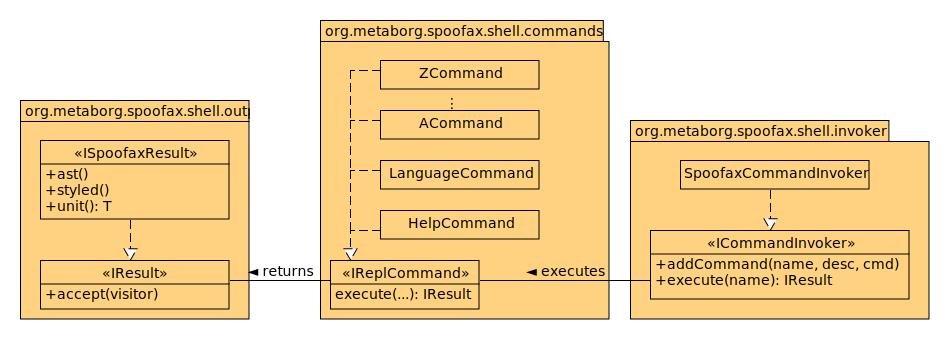
\includegraphics[width=\textwidth]{uml-commands}
  \caption{UML of the commands frontends can execute and the
           corresponding result interfaces.}
  \label{fig:uml-commands}
\end{figure}

Frontends can define additional commands by implementing the
\texttt{IReplCommand} interface.

As explained in the introduction of this chapter, there are only a few
commands that work across all languages, since every language can define its
own transformations or evaluation strategy. Therefore, the
\texttt{LanguageCommand} tries to determine several properties of the loaded
language and adjusts the set of loaded commands accordingly.

By splitting operations in small logical units the design ensures command
classes adhere to the Single Responsibility Principle, which makes all REPL
commands less complex and therefore easier to maintain. The logical units that
make up the commands also ensure a flexible design that can be modified
as the Spoofax architecture develops further on.

%%% Local Variables:
%%% TeX-master: "../main"
%%% End:


\section{}
\label{sec:function-comp}

\begin{figure}[h]
  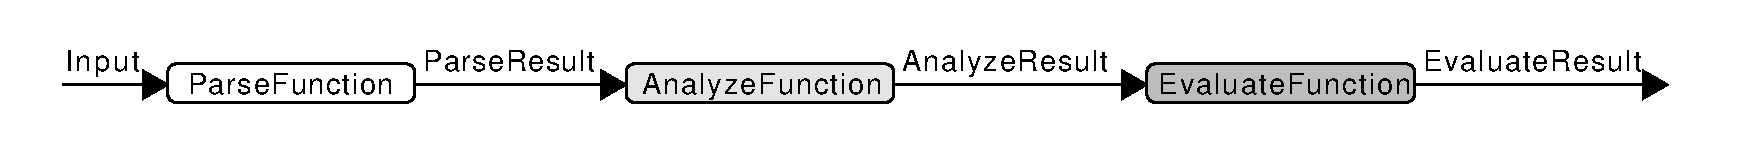
\includegraphics[width=\textwidth]{unit-flow}
  \caption{Processing steps for a language }
  \label{fig:unit-flow}
\end{figure}


\section{Returning Results to the Frontend}
\label{sec:visitor}

As mentioned in \cref{sec:overview}, every command implementing the
\texttt{IReplCommand} interface returns an instance of a class implementing
the \texttt{IResult} interface. It is up to the frontend to determine how to
handle the result. Since commands can result in a failure or an exception (see
\cref{sec:function-comp}), it is not always clear what kind of
\texttt{IResult} the command returns.

To illustrate this, it is possible that a user tries to evaluate an input that
passes the parsing step but fails with an exception at the analyze step (see
\cref{fig:unit-flow}). The expected result is an \texttt{EvaluateResult},
but because an exception was thrown the corresponding wrapped
\texttt{AnalyzeUnit} cannot be created. The command that did the evaluation
then returns a \texttt{FailOrSuccessResult} containing the corresponding
\texttt{ExceptionResult} that caused the failure. However, the caller of the
command has no way of telling that the returned \texttt{IResult} is in fact a
\texttt{FailOrSuccessResult}.

\begin{figure}[t]
  \centering
  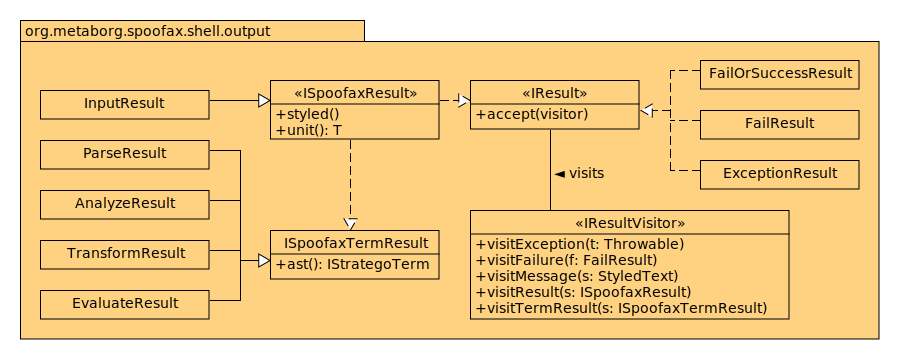
\includegraphics[width=\textwidth]{uml-visitor}
  \caption{UML of the concrete results and the result visitor.}
  \label{fig:uml-visitor}
\end{figure}

The visitor pattern has been adopted to solve this problem. As can be seen in
\cref{fig:uml-visitor}, every \texttt{IResult} can be ``visited'' by classes
implementing the \texttt{IResultVisitor} interface. Each subclass of
\texttt{IResult} decides what visitor method is called, and the
\texttt{IResultVisitor} gets a concrete subclass of \texttt{IResult} as argument
by means of double-dispatch. Furthermore, the \texttt{FailOrSuccessResult}
delegates the visitor to its wrapped \texttt{IResult}.

Implementations of the \texttt{IResultVisitor} can then decide per result type
how to handle the returned information. Since all commands can always return a
result with the original exception or the failed \texttt{ISpoofaxResult} by
returning a \texttt{FailOrSuccessResult}, the frontend is always provided with
error messages or the results of earlier processing steps.

The frontend has the responsibility to decide how to present the returned data
to the user, resulting in a lot of flexibility. However, this flexibility is not
always required. It is not necessary, for example, for a text-based console
REPL, although it can be used to easily highlight errors or print stack
traces. When integrating the REPL in multithreaded graphical user interface
(GUI) toolkits, however, this flexibility is useful.

%%% Local Variables:
%%% mode: latex
%%% TeX-master: "../main"
%%% End:


\section{Evaluation Strategies}
\label{sec:eval-strat}
As explained in \cref{sec:supp-diff-ways}, there are multiple ways for
specifying the dynamic semantics of a language. Interpretation can for example
be performed through an interpreter generated from a DynSem specification, or by
implementing the interpreter in Stratego or Java. However, in the end all of
these methods do the same thing, that is they accept an AST as input and somehow
transform it into an output. In Spoofax, both the input and the output can be
represented as a Stratego term. It is only the internal representation of the
evaluation context and the implementation of the interpreter that is different.

The Strategy pattern is useful for computation task that have the same types of
input and output, but a different implementation. As this is what is the case
for the different methods of evaluation, the method or ``strategy'' of
evaluation is therefore put behind an interface called
\texttt{``IEvaluationStrategy''}. \Cref{fig:uml-eval-strat} shows a UML diagram
of this part of the design.

\begin{figure}[b]
  \centering
  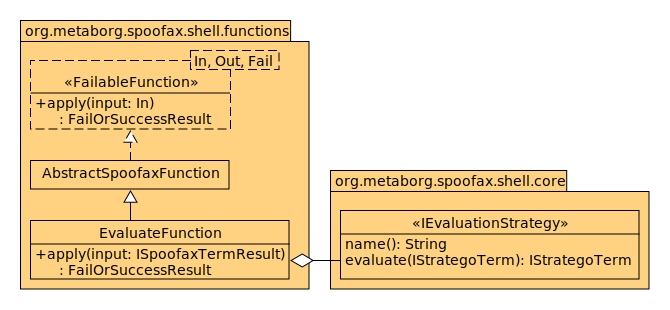
\includegraphics[width=0.8\textwidth]{uml-eval-strat}
  \caption{UML of the \texttt{IEvaluationStrategy} interface and its
    collaborators.}
  \label{fig:uml-eval-strat}
\end{figure}

An implementer of the \texttt{IEvaluationStrategy} is responsible for performing
execution on an AST representation of a program within the evaluation context
that it maintains throughout successive invocations. In this way, maintaining
the evaluation context is encapsulated, and no assumptions are made of what the
evaluation context looks like. This is a desirable property since the
representation of an evaluation context varies across languages and evaluation
methods.

%%% Local Variables:
%%% mode: latex
%%% TeX-master: "../main"
%%% End:


%%% Local Variables:
%%% mode: latex
%%% TeX-master: "main"
%%% End:
